\documentclass{article}
\usepackage{import}
\import{../../../lib/latex/}{wgmlgz}

\begin{document}

\itmo[
       variant=103,
       labn=2,
       worktype=Курсовая работа часть,
       discipline=Дискретная математика,
       group=P3115,
       student=Владимир Мацюк,
       teacher=Поляков Владимир Иванович,
       logo=../../../lib/img/itmo.png
]

\newcommand{\car}{\multicolumn{1}{c@{\hspace*{\tabcolsep}\makebox[0pt]{\curvearrowleft}}}{}}
\newcommand{\rcar}{\multicolumn{1}{c@{\hspace*{\tabcolsep}\makebox[0pt]{\curvearrowright}}}{}}
\newcommand{\ncar}{\multicolumn{1}{c@{\hspace*{\tabcolsep}\makebox[0pt]{}}}{}}
\newcommand{\SPACE}{\multicolumn{12}{c}{}}
\newcommand{\INT}{\multicolumn{5}{c}{\MM{Интерпретации}}}
\newcommand{\PLUS}{\multirow{2}{*}{+}}
\newcommand{\MINUS}{\multirow{2}{*}{-}}
\newcommand{\SIGN}{\multicolumn{2}{c}{\MM{Знаковая}}}
\newcommand{\USIGN}{\multicolumn{2}{c}{\MM{Беззнаковая}}}

\section{Вариант}
$$
C=(A\pm1)_{mod 15}
$$
Число входных/выходных переменных 5/5
Разрядность операндов: 4/-
\section{Задание}

\begin{enumerate}
       \item Построить таблицу истинности системы булевых функций, отражающую закон функционирования комбинационной части операционного
       устройства, реализующего заданные операции.
       \begin{center}
              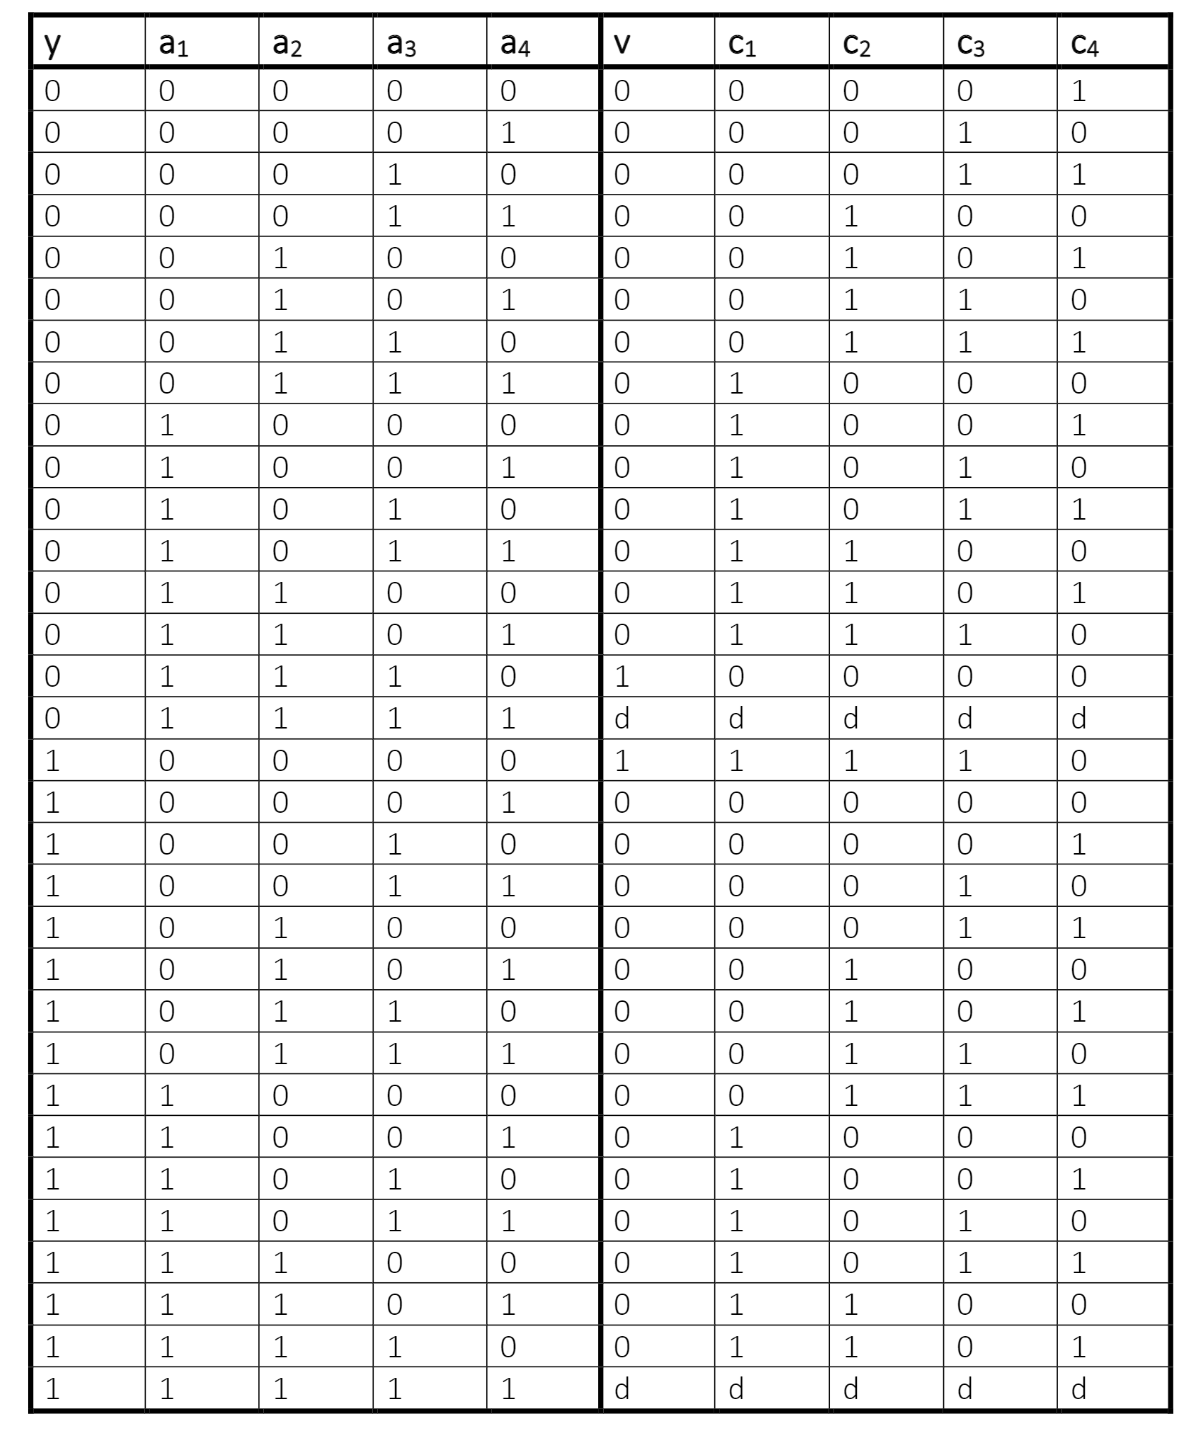
\includegraphics[scale=0.8]{table.png}
       \end{center}
       \item Привести систему булевых функций к виду, дающему минимальную цену схемы, путем решения задач минимизации, факторизации и декомпозиции.

       \begin{center}
              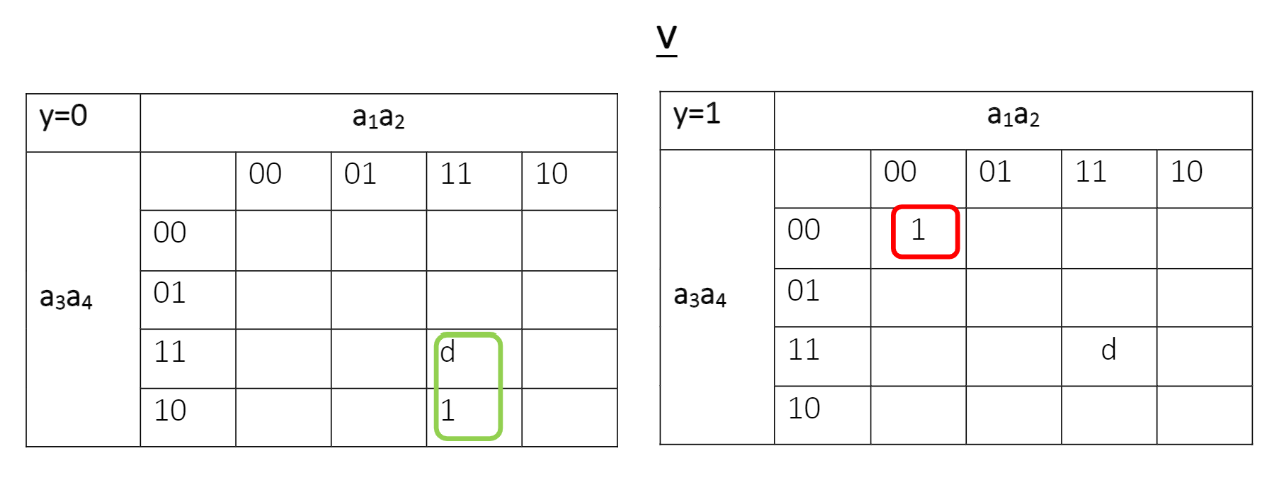
\includegraphics[scale=0.8]{v.png}
              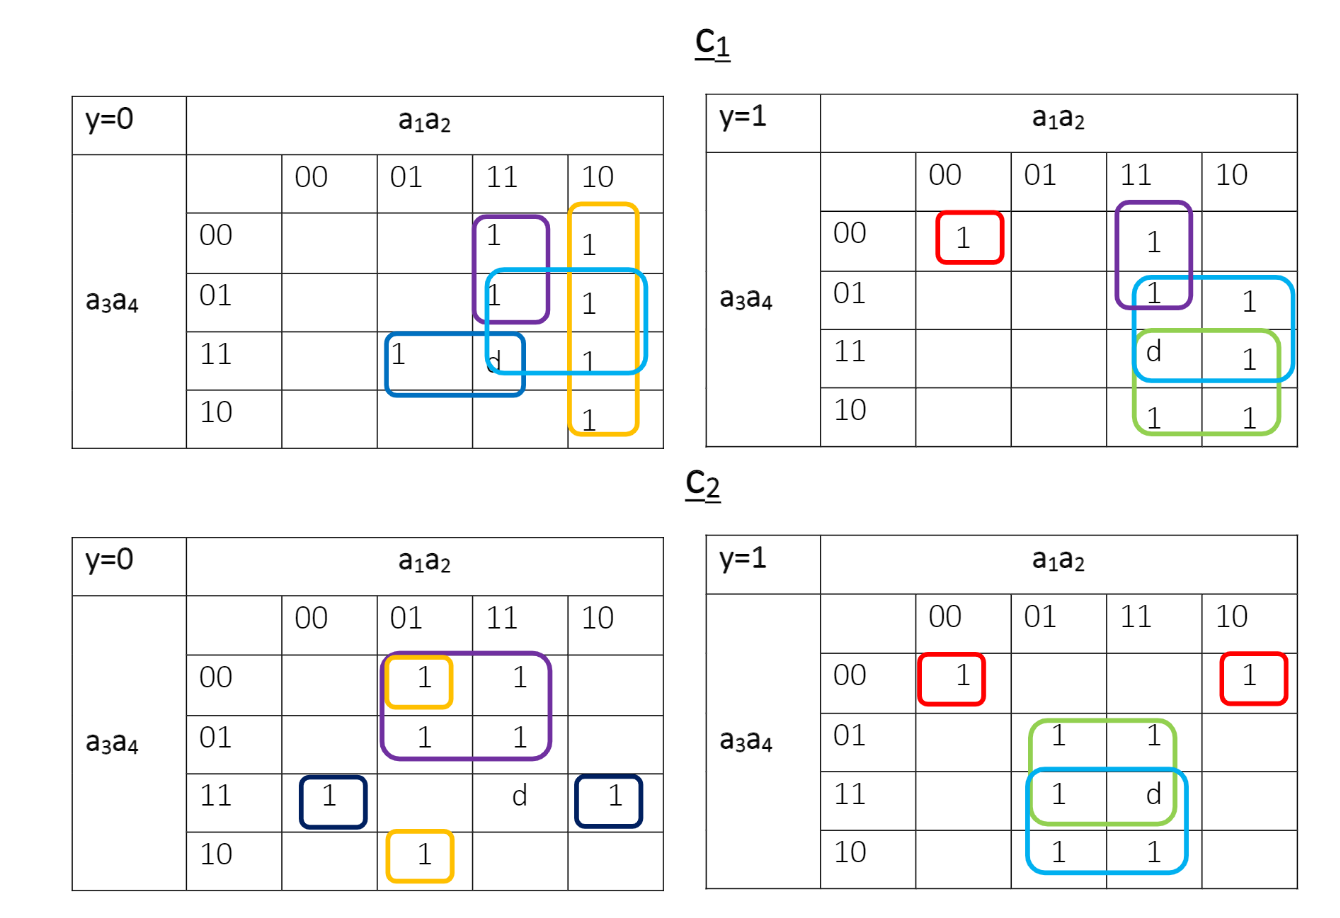
\includegraphics[scale=0.8]{c12.png}
              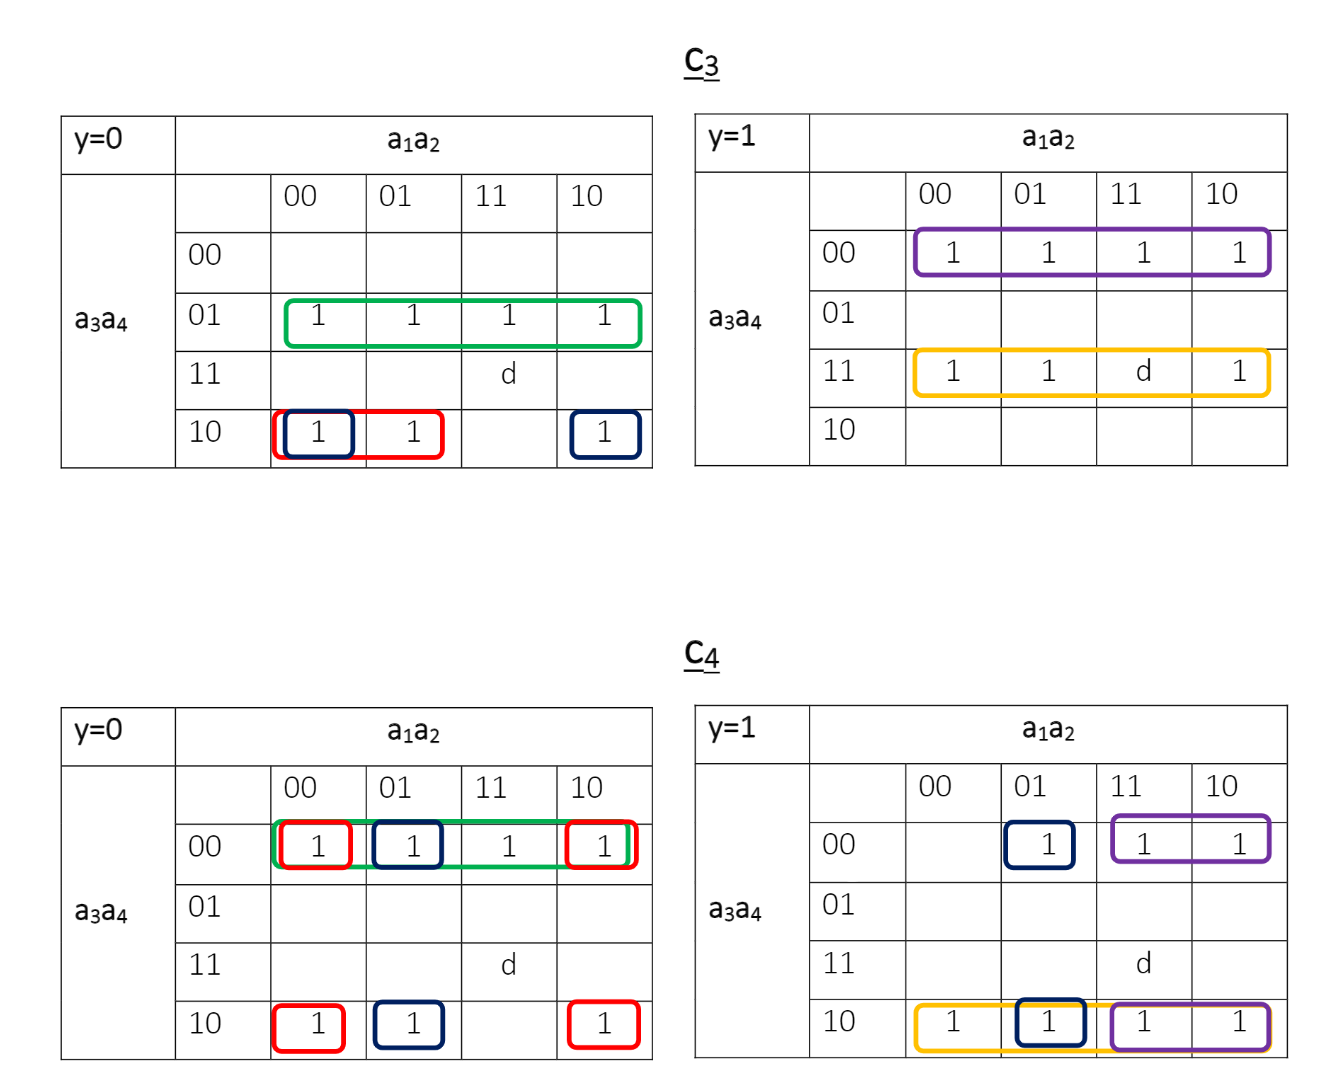
\includegraphics[scale=0.8]{c34.png}
       \end{center}
       
$$\left\{ \begin{array}{l}
       v=  \overline{y}a_1a_2a_3∨y\overline{a_1a_2a_3a_4}\ (S_q=11) \\
       c_1=  \overline{y}a_1\overline{a_2}∨a_1a_2\overline{a_3}∨\overline{y}a_2a_3a_4∨y\overline{a_1a_2a_3a_4}∨ya_1a_3∨a_1a_4\  (S_q=33) \\
       c_2=\overline{y}a_2\overline{a_3}∨\overline{ya_2}a_3a_4∨\overline{ya_1}a_2\overline{a_4}∨y\overline{a_2a_3a_4}∨ya_2a_4∨ya_2a_3\ (S_q=27) \\
       c_3= \overline{ya_3}a_4∨\overline{ya_2}a_3\overline{a_4}∨\overline{ya_1}a_3\overline{a_4}∨y\overline{a_3a_4}∨ya_3a_4\ (S_q=22) \\
       c_4=   \overline{ya_3a_4}∨\overline{ya_2a_4}∨ya_3\overline{a_4}∨ya_1\overline{a_4}∨\overline{a_1}a_2\overline{a_4}\ (S_q=20) \\
\end{array} \right.$$
$$S_q =113$$

$$\left\{ \begin{array}{l}
       φ=y\overline{a_2a_3a_4} (S_q=4) \\
       v=  \bar{y}a_1a_2a_3 ∨φ\bar{a_1} (S_q=8) \\
       c_1=  \overline{y}a_1\overline{a_2}∨a_1a_2\overline{a_3}∨\overline{y}a_2a_3a_4∨φ\overline{a_1}∨a_1ya_3∨a_1a_4\  (S_q=24) \\
       c_2=\overline{y}a_2\overline{a_3}∨\overline{ya_2}a_3a_4∨\overline{ya_1}a_2\overline{a_4}∨φ∨a_2y(a_3∨a_4)\ (S_q=21) \\
       c_3= \overline{ya_3}a_4∨\overline{y}a_3\overline{a_4}(\overline{a_2}∨\overline{a_1})∨ya_3a_4∨y\overline{a_3a_4}\ (S_q=19) \\
       c_4=   \overline{ya_4}(\bar{a_3}∨\bar{a_2})∨y\bar{a_4}(a_3∨a_1)∨\bar{a_1}a_2\bar{a_4}\ (S_q=16) \\
\end{array} \right.$$
$$S_q =92$$
$$Tv=3τ,\ Tc_1=4τ,\ Tc_2=4τ,\ Tc_3=3τ,\ Tc_4=3τ ,\ T= max (Тv, Tc_1, Tc_2, Tc_3, Tc_4)= 4τ.$$

\item Построить комбинационные схемы, реализующие систему булевых
функций на элементах различных базисов. Для каждой схемы определить
цену по Квайну и задержку.
\item Провести анализ построенных схем для различных комбинаций
входных сигналов. 

$$F(00000) = 00001$$
$$F(10000) = 11110$$

\begin{center}
       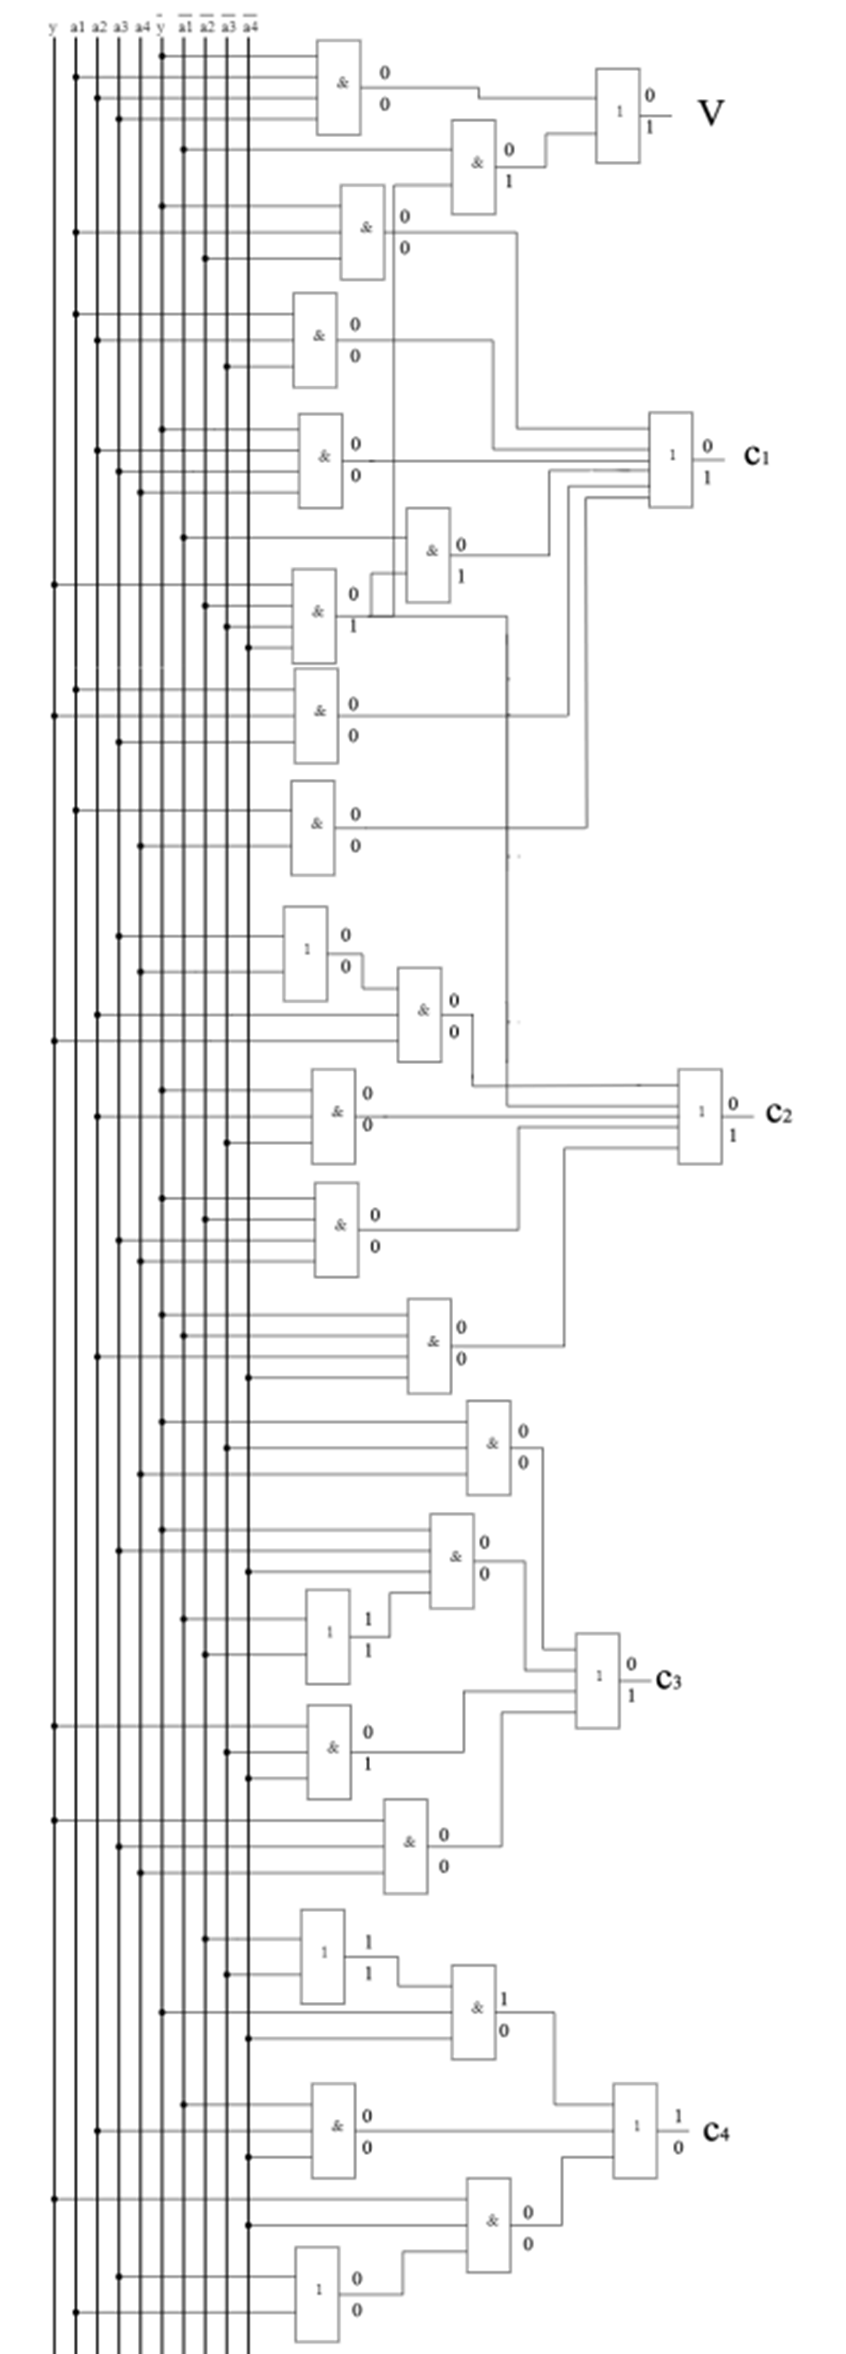
\includegraphics[scale=0.85]{rr.png}
\end{center}


       \end{enumerate}
\end{document}
